
\documentclass[xcolor={dvipsnames}]{beamer}
\usepackage{amsmath,amsfonts,amssymb,pxfonts,eulervm,xspace}
\usepackage{graphicx}
 \usepackage{multimedia}

\graphicspath{{./figures/}}
\usetheme{ccnycrest}
\begin{document}

\title{ CS102: History}
\author{Hannah Aizenman}
\date{haizenman@ccny.cuny.edu}


\begin{frame}
	\titlepage
\end{frame}

\begin{frame}{History of CS: 1805}
	\begin{columns}
	 \begin{column}{.49\textwidth}
	\begin{itemize}
	\item Joseph-Marie Jacquard
	\item punch card programs
	\item programmable loom
	\end{itemize}
 	\end{column}
	 \begin{column}{.49\textwidth}
  		\begin{figure}
 		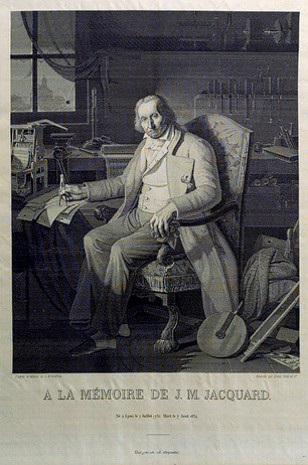
\includegraphics[scale=0.5]{Jacquard_Joseph_Marie_woven_silk}
		\end{figure}
	\end{column}
\end{columns}
\end{frame}

\begin{frame}{History of CS: 1837}
	\begin{columns}
	 \begin{column}{.49\textwidth}
		\begin{center}Charles Babbage\end{center}
		\begin{figure}
		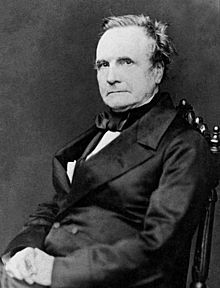
\includegraphics[scale=0.5]{Charles_Babbage}
		\caption{Invented first computer}
		\end{figure}
 	\end{column}
	 \begin{column}{.49\textwidth}
		\begin{center}Ada Lovelace\end{center}
  		\begin{figure}
 		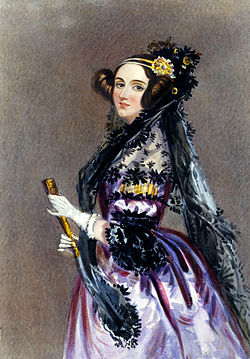
\includegraphics[scale=.60]{Ada_Lovelace_portrait}
		\caption{Wrote first program}
		\end{figure}
	\end{column}
\end{columns}
\end{frame}
\begin{frame}{Difference Engine-Polynomial Calculator}
	\begin{center}
	\href{http://youtu.be/i_u3hpYMySk}{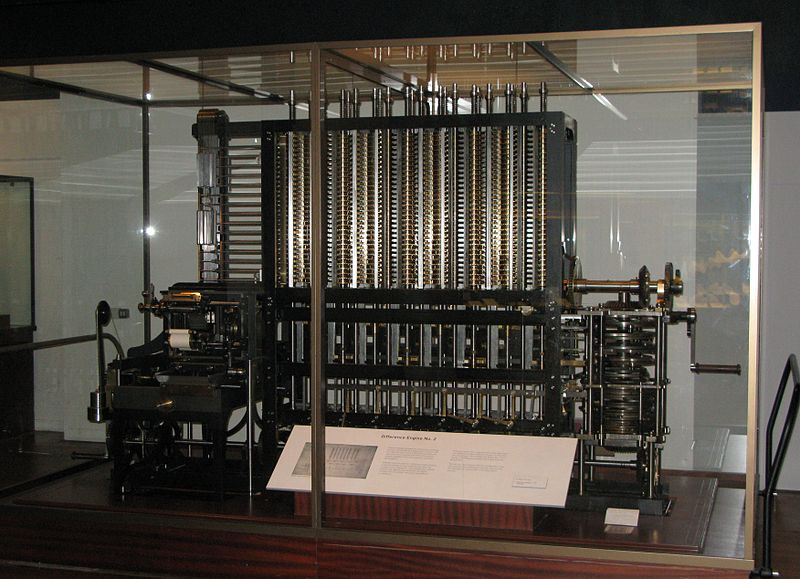
\includegraphics[width=0.8\textwidth]{Babbage_Difference_Engine}}
	\end{center}
\end{frame}

\begin{frame}{History of CS: 1890}
	\begin{columns}
	 \begin{column}{.49\textwidth}
			\begin{center}Herman Hollerith\end{center}
  			\begin{figure}
 				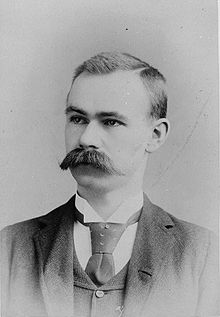
\includegraphics[scale=.50]{Hollerith}
			\end{figure}
 	\end{column}
	 \begin{column}{.49\textwidth}
		\begin{center}Punchcard Tabulator\end{center}
  		\begin{figure}
 		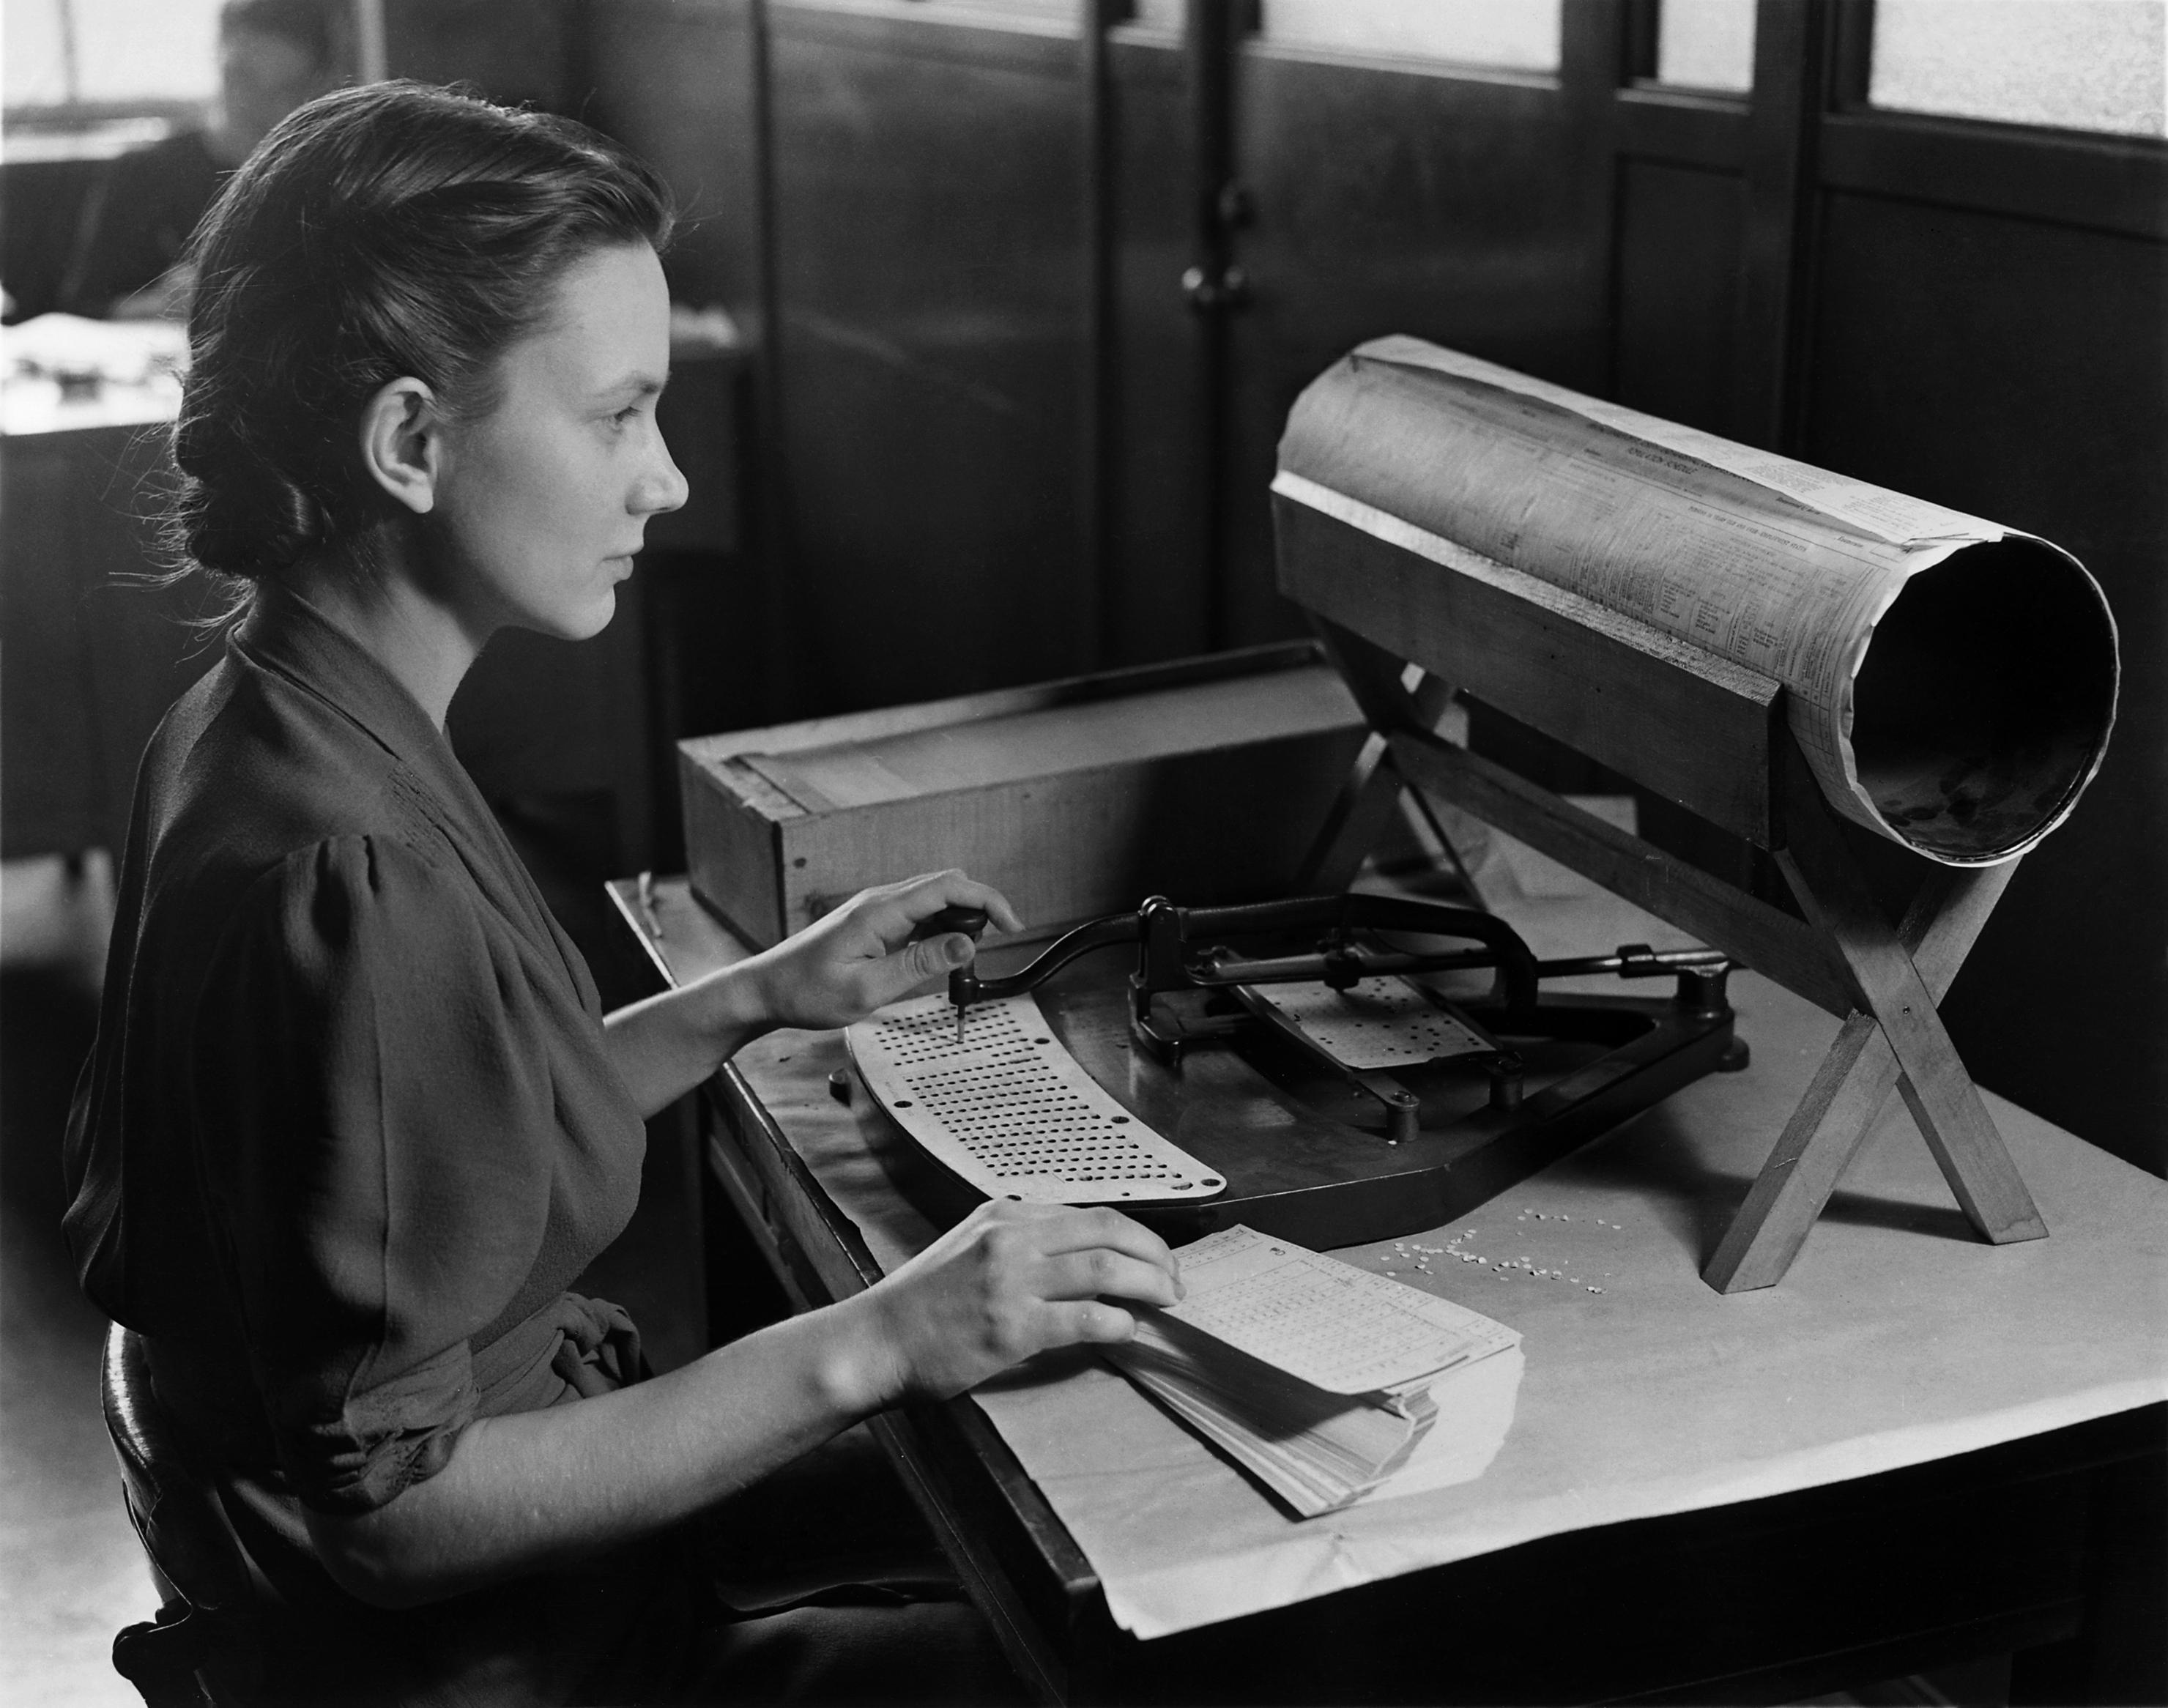
\includegraphics[scale=0.20]{Card_puncher_NARA_513295}
		\caption{Hollerith card puncher used by the United States Census Bureau}
		\end{figure}
	\end{column}
\end{columns}
\end{frame}

\begin{frame}{The Tabulator}
	\begin{center}
	\href{http://channel.nationalgeographic.com/channel/the-link/videos/the-tabulator/}{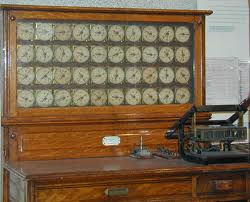
\includegraphics[width=0.8\textwidth] {tabulator}}
	\end{center}
\end{frame}

\begin{frame}{History of CS: WW11}
	\begin{columns}
	 \begin{column}{.49\textwidth}
			\begin{itemize}
				\item Alan Turing
				\item father of theoretical computer science and AI
				\item also code breaker
				\item turing machine reduces computation to lowest level
			\end{itemize}
 	\end{column}
	 \begin{column}{.49\textwidth}
  		\begin{figure}
 		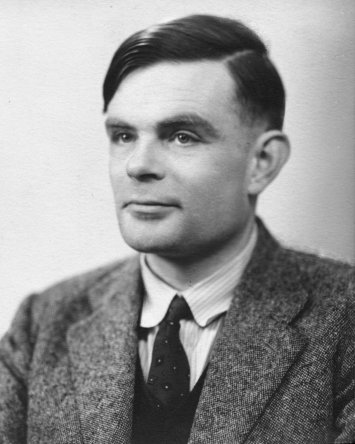
\includegraphics{Alan_Turing_photo}
		\end{figure}
	\end{column}
\end{columns}
\end{frame}

\begin{frame}{Turing Machine}
	\begin{center}
	\href{http://vimeo.com/44202270}{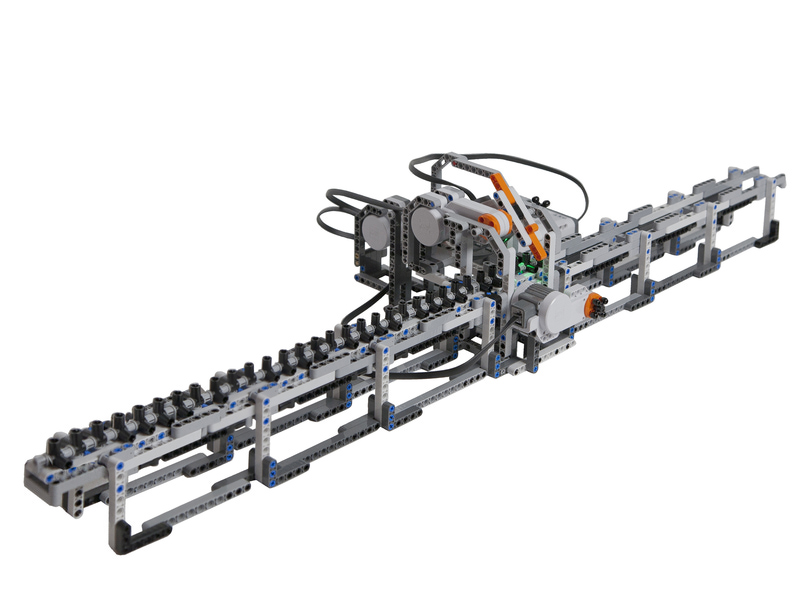
\includegraphics[width=0.8\textwidth]{lego_tm}}
	\end{center}
\end{frame}

\begin{frame}{Why Code?}
\begin{itemize}
	\item work 10 to 100 times faster 
	\item come up with more creative solutions
	\item engineers spend up to \%95 of their time writing code
	\item src: \href{ http://cacm.acm.org/blogs/blog-cacm/166115-why-scientists-and-engineers-must-learn-programming/fulltext}{ACM blog}
\end{itemize}
\end{frame}
\end{document}